\documentclass{article}
\usepackage[pdfcreator={LaTeX}]{hyperref}
\usepackage{graphicx}
\usepackage[utf8]{inputenc} 
\usepackage[ngerman]{babel}

\usepackage[section,toc]{glossaries}\makeglossaries

\newglossaryentry{Regelwerk}{name=Regelwerk,
	plural = Regelwerke,
	description={Regeln eines bestimmten Kartenspiels}
}
\newglossaryentry{Client}{name=Client,
	plural = Clients,
	description={Ein Spieler (bzw. Computer des Spielers) der das Online-Kartenspiel nutzt.}
}
\newglossaryentry{Server}{name = Server,
	description={Rechner, der das Online-Kartenspiel zur Verfügung stellt}
}
\newglossaryentry{Lobby}{name = Lobby,
	description={Ort, an dem Spieler ein Kartenspiel auswählen oder beitreten können}
}
\newglossaryentry{Spielleiter}{name = Spielleiter,
	description={Derjenige, der in der Lobby ein neues Spiel erstellt}
}
\newglossaryentry{Erstellungsfenster}{name = Erstellungsfenster,
	description={Fenster in welchem der Spielleiter das Spiel festlegt.}
}
\newglossaryentry{Wartefenster}{name = Wartefenster,
	description={Fenster auf welchem man sich befindet, während man darauf wartet, 
		dass die Mindestteilemerzahl erfüllt ist und das Spiel gestartet wird. }
}

\begin{document}
\begin{titlepage}

\begin{center}
\textbf{\textsc{\LARGE Pflichtenheft}}

{\large \today}

\vspace{2cm}
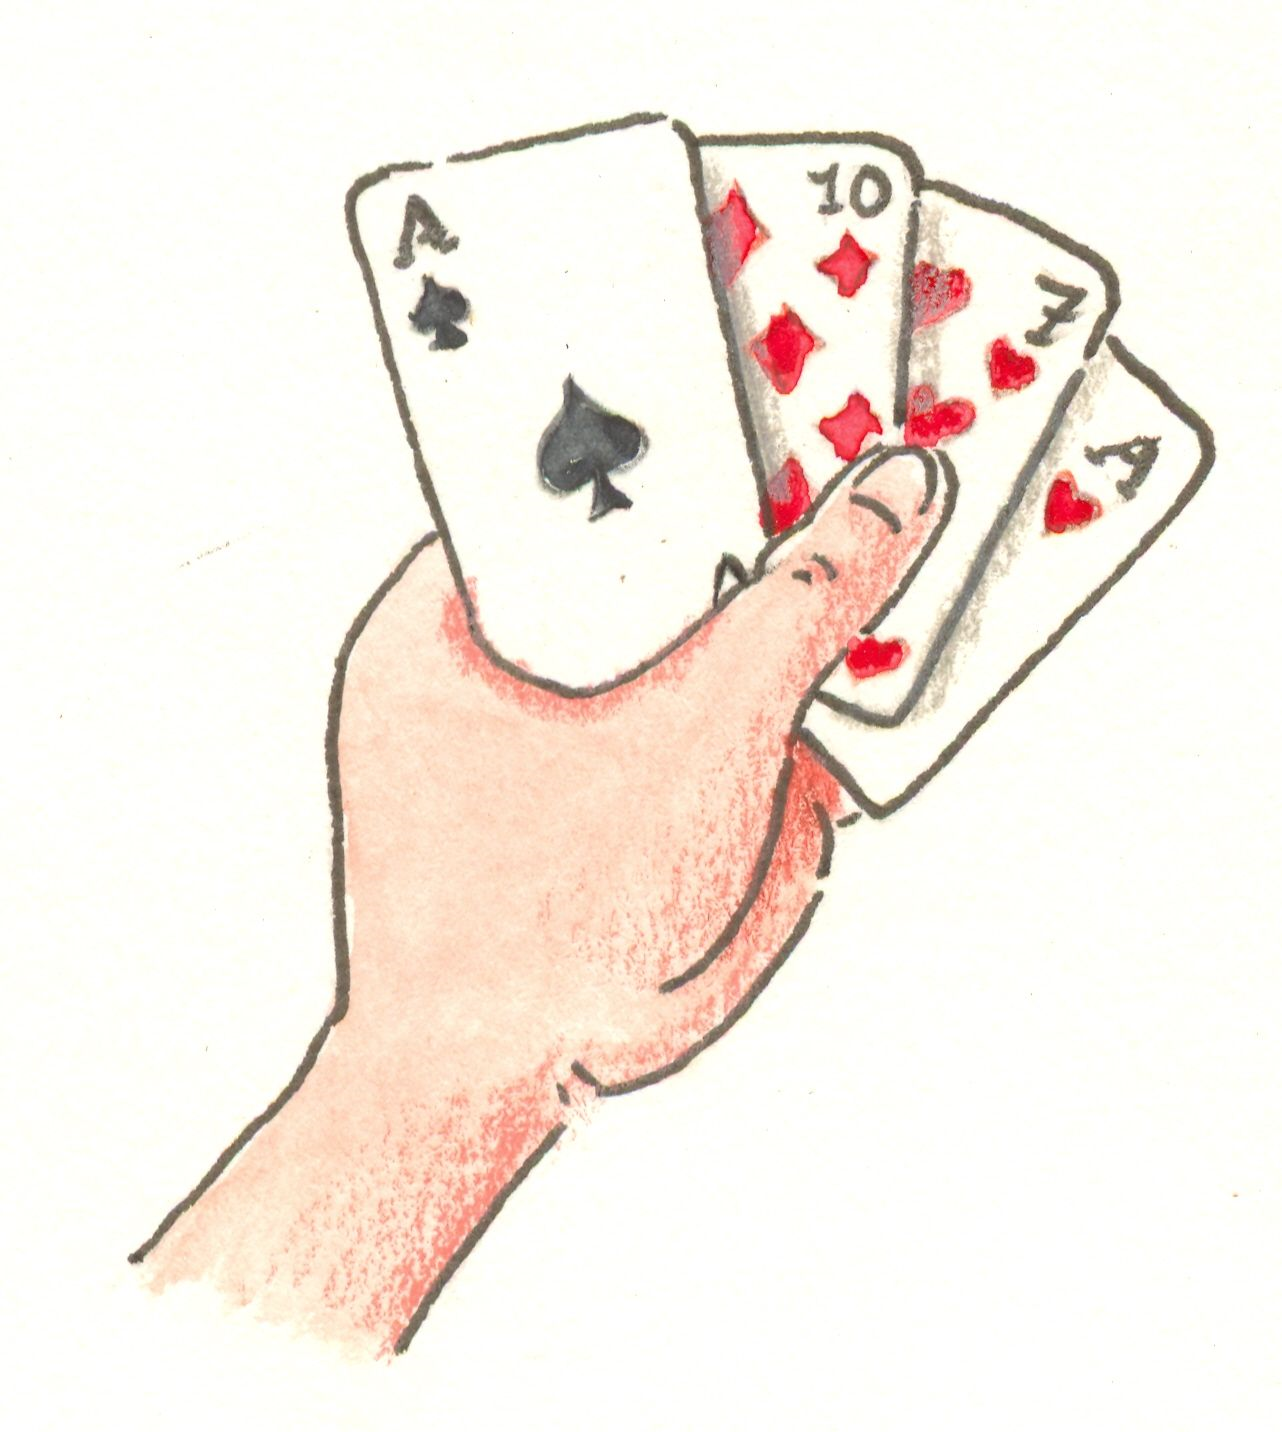
\includegraphics{kartenspiel}

\vspace{2cm}

\begin{tabular}{|c|c|c|}\hline
   Phase & Verantwortlicher & E-Mail \\ \hline\hline
   Pflichtenheft & Alina  Meixl  &  alina@meixl.de \\ \hline
   Entwurf & Viktoria Witka & witkaviktoria@freenet.de \\ \hline
   Spezifikation & Daniel Riedl & dariedl14@yahoo.de \\ \hline
   Implementation & Andreas Altenbuchner& a.andi007@gmail.com\\ \hline
   Verifikation &Patrick Kubin & kubin@fim.uni-passau.de\\ \hline
   Präsentation & w& w\\ \hline
 \end{tabular}

\end{center}

\end{titlepage}


\tableofcontents

\section{Zielbestimmung}
Ein Online-Multiplayer Kartenspiel.

\subsection{Musskriterien}
Es gibt einen \gls{Server} der das Spiel verwaltet und \glspl{Client} die spielen.
\subsubsection{\gls{Server}}
\begin{itemize}
	\item \glspl{Client} können einen Benutzernamen auswählen und sich anschließend mit dem Server verbinden.
		Der Benutzername muss Eindeutig sein, ansonsten wird eine Warnmeldung ausgegeben.
	\item Es gibt eine \gls{Lobby} in der ein Spieler die Möglichkeit hat, Spiele zu erstellen und offenen Spielen beizutreten.
	\item Es gibt einen Chat in der \gls{Lobby}.
	\item Mehrere parallel laufender Spiele auf einem Server werden ünterstützt.
	\item Regelauswertung mit Überprüfung erlaubter Aktionen, Punktezählung und  Kartenausgabe.
	\item Die Spiele Hearts und Wizard sind verfügbar.	
	\item Chat mit Mitspielern während eines Spiels ist möglich.
	\item Schutz vor Cheats (Mehrfachanmeldung?)
\end{itemize}

\subsubsection{\gls{Client}}
\begin{itemize}
	\item GUI
	\begin{itemize}
		\item Darstellungsfenster, das mindestens bei der Auflösung von 1024x768 Bildpunkten benutzt werden kann.
		\item Darstellung des laufenden Spiels. Es wird die eigene Hand offen und die Hände der anderen Spieler verdeckt 					angezeigt. Je nach Spiel gibt es einen allgemeinen Ablagestapel in der Mitte des Spielfeldes oder individuelle 					Ablagestapel vor der Hand des jeweiligen Spielers. Der Zähler für Punktestand, gemachte Stiche, übrige Karten 					etc. befindet sich neben  der Hand des jeweiligen Spielers. Für die Gegenspieler wird zusätzlich der Name über 					der Hand angezeigt.)
		\item Eine Karte wird durch einmaliges Anklicken ausgewählt und durch ein Zweites anklicken abgelegt. Es gibt ein extra 					Fenster um die zu verschiebenden Karten bei Hearts bzw. die Stichansage bei Wizard auszufüren.
		\item Die GUI muss den Benutzer sinnvoll unterstützen und benutzerfreundliche Eingabeelemente anbieten.
		\item Die Darstellung und das Spiel müssen flüssig laufen.
		\item Die GUI darf nicht vom \gls{Regelwerk} abhängen.
		\item Beim Start kann der Spieler einen eindeutigen Benutzernamens auswohlen und die IP des \gls{Server}s angeben
		\item In der \gls{Lobby} werden offene Spiele angezeigt und es gibt die Möglichkeit ein neues Spiel zu erstellen oder 					einem Existierenden beizutreten.
		\item Chat in der \gls{Lobby} und während des Spiels ist möglich
	\end{itemize}
	\item Modell
	\begin{itemize}
		\item Verwaltung der Verbindung mit dem \gls{Server}
		\item Verwaltung des aktuellen Spielzustands (soweit \gls{Client} bekannt)
		\item Vorab-Regelauswertung zur Unterstützung des Nutzers (ungültige Spielaktionen sind nicht durchführbar in der 					GUI)
	\end{itemize}
\end{itemize}

\subsection{Wunschkriterien}
\begin{itemize}
	\item Weitere \glspl{Regelwerk} (Uno, Mau-Mau, Black Jack)
	\item Statistiken, die nach dem Spiel angezeigt werden. Sie zeigen die Plazierung pro Runde.
	\item Mehrere Sprachen werden unterstützt (Deutsch, Englisch, evtl. Bayrisch)
	\item Anpassung der GUI durch Spieler ist möglich (Änderung von Hintergrundbild, Kartenrückseite)
	\item Es gibt die Möglichkeit seinem neu erstellten Spiel einen Namen zu geben
	\item Passwortauswahl um Beitritt zu offenen Spielen einzuschränken ist möglich
	\item Nach jedem Spiel kann entschieden werden, ob eine weitere Runde gestartet werden soll
\end{itemize}

\subsection{Abgrenzungskriterien}
\begin{itemize}
	\item Beitreten eines bereits laufenden Spieles nicht möglich
	\item keine Persistenz der Daten über mehrere Sessions, keine Registrierung
	\item keine KI
	\item Spiel wird nicht fortgesetzt, sobald ein Spieler es verlässt
	\item Es werden nur 3-6 Spieler unterstützt
	\item Es gibt keinen Schimpfwortfilter
\end{itemize}

\section{Produkteinsatz}
\subsection{Anwendungsbereich}
Ein Kartenspiel, welches im Freundeskreis oder mit Fremden über das Intenet gespielt werden kann.
\subsection{Zielgruppe}
Personen, die gemeinsam über ein lokales Netzwerk oder das Internet spielen möchten. 
\subsection{Betriebsbedingungen}
Dauerbetrieb der Software.

\section{Produktumgebung}
\subsection{Software}
	\begin{itemize}
		\item \gls{Client}
		\begin{itemize}
			\item Betriebssystem Microsoft Windows, Mac OS X oder Linux mit aktueller Java Laufzeit.
		\end{itemize}
		\item \gls{Server}
		\begin{itemize}
			\item Betriebssystem Microsoft Windows, Mac OS X oder Linux mit aktueller Java Laufzeit.
		\end{itemize}
	\end{itemize}

\subsection{Hardware}
\begin{itemize}
		\item \gls{Client}
		\begin{itemize}
			\item Internetfähiger Rechner
		\end{itemize}
		\item Server
		\begin{itemize}
			\item Internetfähiger Rechner	
			\item Mindestanforderungen des verwendeten Betriebssystems bezüglich Arbeitsspeicher und Rechenleistung 					      müssen erfüllt sein, können jedoch durch die Anzahl der gehosteten Spieler/Spiele steigen.
		\end{itemize}
	\end{itemize}

\section{Produktfunktionen}
\subsection{Startseite}
\begin{itemize}
	\item /F040/ Auswahl vom gewünschtem \gls{Server} 
	\item /F042/ Auswahl eines Spielernamens
	\item /F045/ Connect mit Weiterleitung zur \gls{Lobby}
	\item /F050W/ Auswahl der Sprache
\end{itemize}

\subsection{\gls{Lobby}}
\begin{itemize}
	\item /F060/ Senden einer Nachricht an andere Spieler über den \gls{Server}
	\item /F070/ Einem Spiel beitreten. (Bei Passwort geschützten Spiel Weiterleitung zur Passwortabfrage ansonsten Weiterleitung zum \gls{Wartefenster})
	\item /F080/ Erstellen eines neuen Spiels (Weiterleitung zum \gls{Erstellungsfenster})
	\item /F90/ Verlassen der \gls{Lobby} (Programmende)
\end{itemize}

\subsection{Erstellungsfenster}
\begin{itemize}
	\item /F120/ Auswahl des \gls{Regelwerk}s
	\item /F122/ Eingabe eines Namens für das zu erstellende Spiel
	\item /F124/ Erstellung abbrechen und \gls{Erstellungsfenster} verlassen (Zurückleitung zur Lobby)
	\item /F126/ Erstellen eines neues Spiels (Weiterleitung zum Wartefenster)
	\item /F128/ Hilfe zum Spiel(Wie?)
	\item /F130W/ Möglichkeit ein Passwort für das Spiel zu setzen
\end{itemize}

\subsection{Passwortabfrage}
\begin{itemize}
	\item /F140W/ Eingabe des Passworts.
	\item /F142/ Einem Spiel beitreten mit Zugang zum \gls{Wartefenster}
	\item /F145/ Abbrechen und zur \gls{Lobby} zurückkehren
\end{itemize}

\subsection{Wartefenster}
\begin{itemize}
	\item Spieler
	\begin{itemize}
		\item /F160/ Chat mit anderen Spielern im selben Spiel
		\item /F170/ Verlassen des Spiels (Zurückleitung zur Lobby)
	\end{itemize}
	\item Spielleiter
	
	Besitzt alle Funktionen des Spielers
	\begin{itemize}
		\item /F180/ Spieler entfernen
		\item /F190/ Auflösung des Spiels durch Verlassen des Wartefensters
		\item /F200/ Starten des Spiels (Voraussetzung: Mindestanzahl der Spieler erreicht)
	\end{itemize}
\end{itemize}

\subsection{Spiel}
\begin{itemize}
	\item Alle Spiele
	\begin{itemize}
		\item /F210/ Verlassen des Spiels (Folge: Alle Spieler kehren zur Serverlobby zurück)
		\item /F220/ Nachricht senden an andere Spieler
		\item /F225/ Karte auswählen (Voraussetzung: Am Zug und Karte erlaubt zu spielen)
		\item /F230/ Karte spielen (Voraussetzung: Karte ausgewählt)
	\end{itemize}
	\item Herz
	\begin{itemize}
		\item /F260/ Auswahl der Karten, die weitergeschoben werden sollen.
	\end{itemize}
	\item Wizard
	\begin{itemize}
		\item /F360/ Auswahl der Trumpffarbe zu Beginn einer Runde (Voraussetzung: Aufdecken des Zauberers)
		\item /F370/ Eingabe der gewünschten Stiche zu Beginn jeder Runde
	\end{itemize}
\end{itemize}

\section{Produktdaten}
\subsection{\gls{Regelwerk}e}
\subsubsection{/D010/ Hearts}	
\begin{itemize}
	\item Kartenstapel
	\begin{itemize}
		\item Kartenanzahl: 52
		\item Karten:
		\begin{itemize}
			\item Farbe: Kreuz, Pik, Herz, König
			\item Wertigkeit: 2-10,Bube,Dame,König,Ass
			\item Punkte: Herz = 1 Punkt, Pik Dame = 13 Punkte, andere = 0 Punkte
		\end{itemize}	
		\item Kartenverteilung pro Runde: 13 Karten				
	\end{itemize}
	\item Erlaubte Spieleranzahl: 4 Spieler		
	\item Spieler /D010/
	\begin{itemize}
		\item Karten
		\item Punktestand (Bei 100 Punkte Spielende)
		\item Pik 2 Regel (Muss bei Besitz gespielt werden)
		\item Status (Am Zug, Wartend)
	\end{itemize}
	\item Runden
	\item Tauschreihenfolge	
	\item Ablagestapel:
	\begin{itemize}
		\item Zugreihenfolge
		\item Spielbare Karten
		\item Stichvergabe an Spieler
		\item Anzeigedauer der Karten
	\end{itemize}
	\item Platzierung der Spieler
\end{itemize}
	
\subsubsection{/D020/ Wizard}
\begin{itemize}
	\item Kartenstapel
	\begin{itemize}
		\item Kartenanzahl: 60
		\item Karten
		\begin{itemize}
			\item Reguläre Karten
			\begin{itemize}
				\item Farbe: blau,rot,grün,gelb
				\item Wertigkeit: 1-13	
			\end{itemize}
			\item Sonderkarten
			\begin{itemize}
				\item Zauberer: 4 Karten
				\item Narr: 4 Karten
			\end{itemize}			
		\end{itemize}	
		\item Kartenverteilung pro Runde: 1 plus eine für jede weitere Runde
	\end{itemize}
	\item Spieleranzahl: 3-6
	\item Spieler /D010/
	\begin{itemize}
		\item Karten
		\item Stiche
		\item Stichvorhersage
		\item Status (Am Zug, Wartend)
	\end{itemize}
	\item Runden
	\begin{itemize}
		\item Anzahl: 20,15,12,10 (Abhängig von Spieleranzahl)
		\item Trumpffarbe
		\item Anfangsspieler
		\item Spielende bei letzter Runde
	\end{itemize}
	\item Ablagestapel
	\begin{itemize}
		\item Zugreihenfolge
		\item Spielbare Karten
		\item Stichvergabe an Spieler
		\item Anzeigedauer der Karten
	\end{itemize}
	\item Platzierung der Spieler
\end{itemize}

\subsection{Andere Daten}
\subsubsection{/D030/ Spieler}
\begin{itemize}
	\item Spielername(eindeutig)
	\item Server
	\item Sprache
	\item Status(\gls{Lobby}, Spiel)
\end{itemize}	

\subsubsection{/D040/ Spiel}
\begin{itemize}
	\item Spielname(eindeutig)
	\item Spieler /D030/
	\begin{itemize}
		\item \gls{Spielleiter}
		\item Andere Spieler
	\end{itemize}
	\item Spieleranzahl
	\item Regelwerk /D010/ oder /D020/
	\item Chatinhalt
	\item Status(Erstellung,Laufend,Ende)
	\item Passwort(optional)
\end{itemize}

\subsubsection{/D050/ \gls{Lobby}}
\begin{itemize}
	\item Spieler /D010/ (Status = \gls{Lobby})
	\item Spiele /D040/ (Status = Erstellung)
	\item Chatinhalt
\end{itemize}

\subsection{Andere Daten}
\subsubsection{/D030/ Spieler}
\begin{itemize}
	\item Spielername(eindeutig)
	\item Server
	\item Sprache
	\item Status(Lobby, Spiel)
\end{itemize}	

\subsubsection{/D040/ Spiel}
\begin{itemize}
	\item Spielname(eindeutig)
	\item Spieler /D030/
	\begin{itemize}
		\item Spielleiter
		\item Andere Spieler
	\end{itemize}
	\item Spieleranzahl
	\item Regelwerk /D010/ oder /D020/
	\item Chatinhalt
	\item Status(Erstellung,Laufend,Ende)
	\item Passwort(optional)
\end{itemize}

\subsubsection{/D050/ Lobby}
\begin{itemize}
	\item Spieler /D010/ (Status = Lobby)
	\item Spiele /D040/ (Status = Erstellung)
	\item Chatinhalt
\end{itemize}


\section{Produktleistungen}
\subsection{\gls{Lobby}}
\begin{itemize}
	\item /L100/ Anzeige von eingeloggten Spielern
	\item /L110/ Anzeige von erstellten Spielen	
	\item /L115/ Anzeige des Chatdialoges		
\end{itemize}

\subsection{Erstellungsfenster}
\begin{itemize}
	\item /L120/ Anzeige eines Spiellogos
	\item /L122/ Anzeige einer kurzen Spielbeschreibung (bei Mouseover über das Logo)
\end{itemize}

\subsection{Wartefenster}
\begin{itemize}
	\item /L150/ Anzeigen des Spieltyps
	\item /L155/ Anzeigen der Mitspieler
	\item /L158/ Anzeige des Chatdialoges
	\item /L160/ Ab Mindestanzahl der Spieler kann der Spielersteller des Spiel starten ???
	\item /L170/ \gls{Wartefenster} wird nur aufgelöst wenn der Spielersteller selbst das Spiel verlässt ???
\end{itemize}

\subsection{Spiel}
\begin{itemize}
	\item /L190/ Anzeige der eigenen Karten
	\item /L192/ Anzeige der verdeckten Karten der Mitspieler
	\item /L194/ Anzeige des Ablagestapels
	\item /L195/ Anzeige des Aufnahmestapels
	\item /L195/ Anzeige der Anzahl der restlichen Karten für jeden Spieler bzw. Anzahl der vorhergesagten Stiche
	\item /L200/ Anzeige des Punktestandes
	\item /L250/ Anzeige einer Auswertung nach Beendigung einer Runde oder eines Spiels
	\item /L260/ Anzeige des Chatdialoges
	\item /L270/ Nutzen des Chatdialoges zur Benachrichtigung der Spieler über Ergebnisse und Spielstand
\end{itemize}
	
\subsection{Allgemein}
\begin{itemize}
	\item /L280/ Einhaltung der Spielregeln gewährleisten
	\item /L290/ Fehlermeldungen akkumuliert ausgeben
	\item /L300/ Verwaltung mehrerer parallel laufender Spiele
	\item /L310/ Chat und Spiel sollen flüssig laufen
	\item /L320/ Einfache und hilfreiche Bedienbarkeit
	\item /L330/ Schutz vor Cheats
	\item /L340/ Verhinderung langer Wartezeiten
	\item /L350W/ Mehrsprachigkeit unterstützen
\end{itemize}

\section{Benutzeroberfläche}
\begin{itemize}
	\item Startseite:  Auf dieser Seite kann sich der Spieler einen Benutzernamen aussuchen und sich mit dem Server verbinden.\\ 				\ \\
		\makebox[\textwidth]{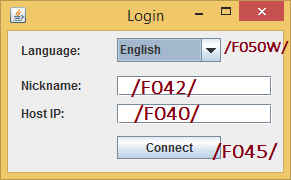
\includegraphics{GUI_images/Login}}
		\ \\
	\item \gls{Lobby}: In der \gls{Lobby} konnen Spieler mit den unteren Buttons ein neues Spiel erstellen,  einem offenem Spiel 					beitreten oder die \gls{Lobby} verlassen. In der linken Spalte sind die Spieler zu sehen, die sich gerade in der 					\gls{Lobby} befinden (wobei für jeden Spieler eine Statusmeldung angezeigt wird). In der rechten Spalte sieht 					man die offenen Spiele, mit momentaner Spielerzahl und und Spieltyp. Im unteren Teil der Lobby ist der Chat.\\
		\ \\
		\makebox[\textwidth]{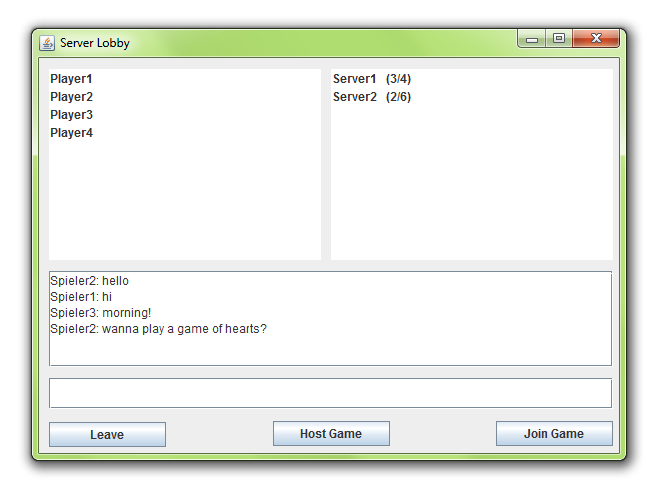
\includegraphics[scale=0.7]{GUI_images/ServerLobby}}
		\newpage
	\item \gls{Erstellungsfenster}: Im \gls{Erstellungsfenster} kann der \gls{Spielleiter} ein neues Spiel erstellen. Dabei muss er ein 			\gls{Regelwerk} aussuchen, und kann wahlweise dem Spiel einen Namen geben und das Passwort setzen. \\
		\ \\
		\makebox[\textwidth]{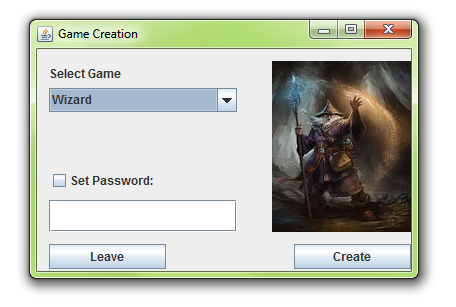
\includegraphics[scale=0.8]{GUI_images/CreateGame}}
		\ \\
	\item \gls{Wartefenster}: Im \gls{Wartefenster} befinden sich die Personen, die einem offenem Spiel beigetreten sind. Sobald 					die Midestspielerzahl erreicht ist kann ein neues Spiel gestartet werden. Für das Wartefenster ist ein eigener 					Chat verfügbar. Man kann das Wartefenster auch mit einem der unteren Buttons verlassen. \\
		\ \\
		\makebox[\textwidth]{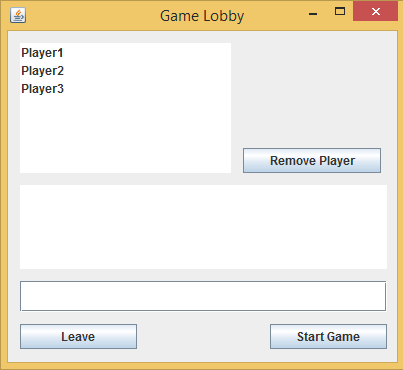
\includegraphics[scale=0.7]{GUI_images/GameLobby}}
		\ \\
	\item Passwortabfrage: Bevor die Spieler einem offenen Spiel beitreten können, müssen sie das Passwort, dass der 						\gls{Spielleiter} festgelegt hat, in das Textfeld eingeben.\\
		\ \\
		\makebox[\textwidth]{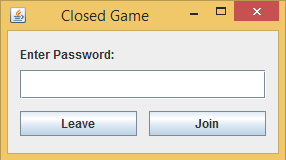
\includegraphics{GUI_images/PasswordRequest}}
		\ \\
	\item Spiel: Im Spielfeld wird die eigene Hand offen, und die der anderen Spieler verdeckt angezeigt. Je nach Spiel gibt es 					einen allgemeinen Ablagestapel in der Mitte des Spielfeldes oder individuelle Ablagestapel vor der Hand des 					jeweiligen Spielers. Der Zähler für Punktestand, gemachte Stiche, übrige Karten etc. befindet sich neben  der 					Hand des jeweiligen Spielers. Für die Gegenspieler wird zusätzlich der Name über der Hand angezeigt.\\
			Im unteren bereich gibt es ein Chatfenster für die Mitspieler.\\
		\ \\
		\makebox[\textwidth]{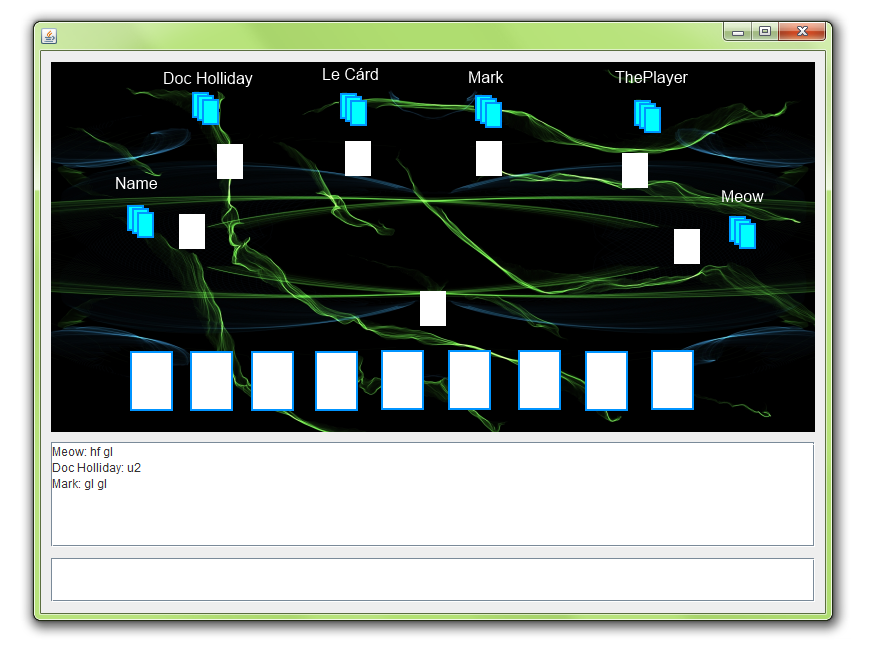
\includegraphics[scale=0.6]{GUI_images/GameClient}}
\end{itemize}

\section{Testszenarien}
\begin{itemize}
	\item Startseite (keine Vorraussetzungen): \\
	\begin{itemize}
	
		\item /T020/ \textit{Verbindungsaufbau mit Server:} Mr. Blue gibt den Nickname "MrBlue" und die Adresse des servers ein (/F040/). Er verbindet sich mit dem Server und gelangt die Lobby (/F045/). 
		
		\item /T030/ \textit{Auswahl der Sprache:} \\ Mr. Blue wählt im Dropdown-Menü die Sprache "English" aus. (/F050W/).
			  
			  
	\end{itemize}

	\item Server Lobby (Vorraussetzungen: /T020/: \\ \\
	\begin{itemize}
	
		\item /T040/ \textit{Spielerliste:} Der eigene Benutzername "MrBlue" und die Benutzernamen aller anderen verbundenen Clients werden sofort in der Spielerliste angezeigt (/L100/).
		
		\item /T050/ \textit{Serverliste:} Alle von Nutzern erstellten Spiele werden in der Spielliste angezeigt (/L110/).
	
		\item /T060/ \textit{Chatnachricht senden:} Mr. Blue gibt die Nachricht "Hallo Kartenwelt!" in das untere Textfeld ein und drückt die Entertaste (/F060/).
		
		\item /T070/ \textit{Chatdialog anzeigen:} Im oberen Textfeld wird die aktuellste Nachricht und alle bisher gesendeten Nachrichten angezeigt (/L115/).
		
		\item /T080/ \textit{Spiel erstellen:} Mr. White erstellt ein Spiel und gelangt ins Erstellungsfenster (/F080/).
		
		\item /T085/ \textit{Mehrere Spiele erstellen (Vorrausetzung: /T080/, /T110/):} Mr Pink erstellt ein weiteres Spiel und gelangt ins Erstellungsfenster (/F080/).
		
		\item /T090/ \textit{Spiel beitreten:} Mr. Blue tritt dem bereits korrekt geöffneten und noch nicht vollen Spiel von Mr. White bei und gelangt ins Wartefenster (/F070/). Die Lobby bleibt geöffnet.
		
		\item /T095/ \textit{Passwortabfrage:} Das Spiel von Mr. White is passwortgeschützt. Mr. Blue gibt "youshouldtip" in das zugehörige Textfeld ein (/F140/) und drückt den 'Join'-Knopf, wodurch er zum Wartefenster weitergeleitet wird (/F142/). 
		
		\item /T097/ \textit{Passwortabfrage(Abbruch):} Das Spiel von Mr. White ist passwortgeschützt. Mr. Blue kennt das Passwort nicht, also drückt er den 'Cancel'-Knopf und gelangt zurück in die Lobby (/F145/).
			  
	\end{itemize}
	
	\item Erstellungsfenster (Vorraussetzung: /T080/): 
	
	\begin{itemize}
	
		\item /T100/ \textit{Regelwerk auswählen:} Mr. White wählt 'Wizard' als Regelwerk aus (/F120/) und schaut sich dessen Logo an (/L120/), sowie eine kurze Beschreibung des Spiels, die erscheint, wenn er mit der Maus über das Logo fährt (/L122/)
		
		\item /T110/ \textit{Spiel erstellen:} Mr. White gibt "NewHeist" als Spielname ein (/F122/) und legt die Spielerzahl auf '4' fest (/F???/). Er setzt einen Haken bei 'Passwort' und gibt "youshouldtip" als Passwort ein (/F130W/). Er drückt auf den 'Create'-Knopf, erstellt somit ein Spiel und wird zum Wartefenster weitergeleitet (/F126/).
		
		\item /T120/ \textit{Erstellung abbrechen:} Mr. White sieht, dass Mr. Pink schon in einem anderen Spiel ist und entschließt sich die Erstellung abzubrechen. Er drückt den 'Cancel'-Knopf und gelangt zurück in die Lobby (/F124/).
	
	\end{itemize}
	
	\item Wartefenster (Vorraussetzung: /T110/, /T090/)
	
	\begin{itemize}
		
		\item /T130/ \textit{Chat:} Mr. Pink und Mr. White befinden sich im Wartefenster des Spiels. Mr. Pink schreibt die Chatnachricht "Hello Mr. White" und sie wird bei beidem im Chat angezeigt (/F160/).
		
		\item /T170/ \textit{Verlassen:} Mr. Brown ist gerade dem Spiel beigetreten und verlässt es sofort wieder. Er gelangt zurück in die Lobby (/T170/).
		
		\item /T180/ \textit{Spieler entfernen:} Mr. Blue tritt dem Spiel bei. Mr. Pink hat das Spiel erstellt. Er ist somit Spielleiter und entschließt sich dazu Mr. Blue aus dem Spiel zu werfen (/F180/). 
		
		\item /T190/ \textit{Spiel starten:} Mr. Brown und Mr. Orange treten dem Spiel bei. Es sind nun genug Spieler vorhanden und der 'Start'-Knopf ist nicht mehr ausgegraut, deshalb entschließt sich Mr. Pink dazu, das Spiel zu starten (/F200/).
		
		\item /T200/ \textit{Spiel auflösen:} Es dauert Mr. Pink zu lange, bis genug Spieler zusammenkommen, also verlässt er das Wartefenster. Da er der Spielleiter war wird das Spiel aufgelöst und alle Spieler gelangen zurück zur Lobby (/F190/).
		 
	\end{itemize}
	
	\item Spiel spielen 
\end{itemize}

\section{Entwicklungsumgebung}
\subsection{Software}
\begin{itemize}
	\item LaTeX
	\item Eclipse
	\item IBM Rational Software Architect
	\item Git
\end{itemize}

\subsection{Hardware}
\begin{itemize}
	\item Rechner im CIP Pool	
	\item Private Rechner
\end{itemize}

\section{Ergaenzung}
..... 
\newpage
\printglossaries
\end{document}
